\hypertarget{grayscalecolor_8cpp}{}\section{Файл Projects/labs/course\+\_\+project\+\_\+cg/src/image/grayscalecolor.cpp}
\label{grayscalecolor_8cpp}\index{Projects/labs/course\+\_\+project\+\_\+cg/src/image/grayscalecolor.\+cpp@{Projects/labs/course\+\_\+project\+\_\+cg/src/image/grayscalecolor.\+cpp}}
{\ttfamily \#include \char`\"{}grayscalecolor.\+h\char`\"{}}\\*
Граф включаемых заголовочных файлов для grayscalecolor.\+cpp\+:\nopagebreak
\begin{figure}[H]
\begin{center}
\leavevmode
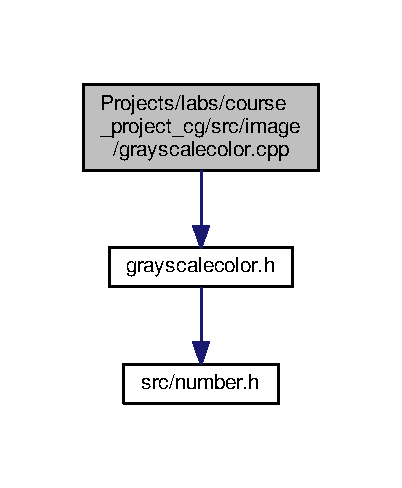
\includegraphics[width=193pt]{d0/d2f/grayscalecolor_8cpp__incl}
\end{center}
\end{figure}
